\documentclass[runningheads,a4paper]{./llncs2e/llncs}

\usepackage{graphicx}
\usepackage{caption}
\usepackage{subcaption}
\usepackage{amssymb}
\setcounter{tocdepth}{3}
%\usepackage{fixltx2e}
\usepackage{mathtools}
\usepackage[nolist,nohyperlinks]{acronym}
% Maintain images and tables within their respective sections
\usepackage[section,subsection,subsubsection]{extraplaceins}
\usepackage{epstopdf}
\usepackage[utf8]{inputenc}
\usepackage{listings}
\usepackage[usenames,dvipsnames]{color}
\usepackage{url}
\usepackage{lipsum}

\setcounter{secnumdepth}{3}

% 
% Change the margins
% 
% \usepackage[margin=2.9cm]{geometry}

\begin{document}
\title{Procedural Generation}

\subtitle{Your Thesis subtitle}
\author{Artur Alkaim \and António Leitão}

\institute{Instituto Superior Técnico, Universidade de Lisboa
\path|{arturalkaim, antonio.menezes.leitao}@tecnico.ulisboa.pt|
\url{http://tecnico.ulisboa.pt/}}

\toctitle{Procedural Generation}
\tocauthor{Artur Alkaim, António Leitão}
\maketitle

%!TEX root = ../report.tex

% 
% Abstract 
% 

\begin{abstract}

% `` The existing CAD tools are geared for manual use. Unfortunately, the manual production of large amounts of complex architectural forms is very time consuming. Procedural generation of these forms is one of the approaches which considerably speed up this process . This approach is the algorithmic construction of these forms , using grammars forms , L -systems , Automatic Phones, etc. This thesis aims to exploit these techniques and their implementation in Rosetta tool. The assessment may include generation of urban environments , buildings and ornaments according to a certain style arquitectónico.``

The existing graphic creation tools are geared for manual use. Unfortunately, the manual production of large amounts of complex architectural forms is very time consuming. Procedural generation of these forms is one of the approaches which considerably speed up this process. This approach consists in the algorithmic construction of these forms through diferent techniques like shape grammars, L-Systems, etc. This project aims to explore this approach and apply it to the procedural modeling of cities by the development of a tool that, in connection with the Rosetta tool, will provide a new mean for the users to explore this approach.


\end{abstract}
%!TEX root = ../report.tex

% 
% Keywords 
% 

\begin{keywords}

Lorem ipsum dolor sit amet, consectetur adipisicing elit, sed do eiusmod
tempor incididunt ut labore et dolore magna aliqua. 

\end{keywords}
%!TEX root = ../report.tex

% 
% Introduction
% 

\section{Introduction (2/3pgs)}

General description of the problem and its context, current solutions, and road map of the project.

(\dots)

\subsection{Procedural Generation} % (fold)
\label{sub:procedural_generation}


As technology evolves and people get new and more powerful devices, they want to take advantage of that with more detailed and complex contents to have more realistic experiences. 
And this is observable in the graphic contents. With more de definition of the screens and the computational power of the machines beating records, the graphic content have to follow up that characteristics in quantity as well as in quality. The issue is that the manual content generation takes a long work time from artists to achieve this quality.
The obvious answer to this problem is to contract more artists to each project to increase the production, but experience have shown that this solution is not scalable, that means that double the number of artists working in a project will not double their overall productivity. And this solution have a big impact on costs, that would take immediately out of the market new producers with less resources.

There is a area of research that tries to solve this problem with \emph{Procedural Content Generation}, or \emph{Procedural Generation}.

Procedural Generation is the algorithmic generation of content in stead of the usual manual creation of content. This can be applied in almost all forms of content, but is mostly used in graphics creation and sound (music and synthetic speech).
``The key property of procedural generation is that in describes the data entity, be it geometry, texture or effect, in terms of a sequence of generation instructions rather than as a static block of data.''\cite{Kelly} This allows anyone with less resources to produce high detailed, and high quality content.

%!TEX root = ../report.tex

\subsection{Procedural Modelling Techniques} % (fold)
\label{sub:procedural_modelling_techniques}

\subsubsection{Fractals} % (fold)
\label{ssub:fractals}


A fractal is a never-ending pattern. Fractals are infinitely complex patterns that are self-similar across different scales. 
This concept is observed in some forms that exist in nature. From trees, mountains, coastlines to the network of neurons on a human cortex can be seen as examples of fractals. Natural shapes tend to be irregular and fragmented and exhibit a complexity incomparable to regular geometry [Mandelbrot 1982]. The Figure~\ref{fig:NFractals} shows some examples of that. 



\begin{figure}
        \centering
        \begin{subfigure}[b]{0.4\textwidth}
                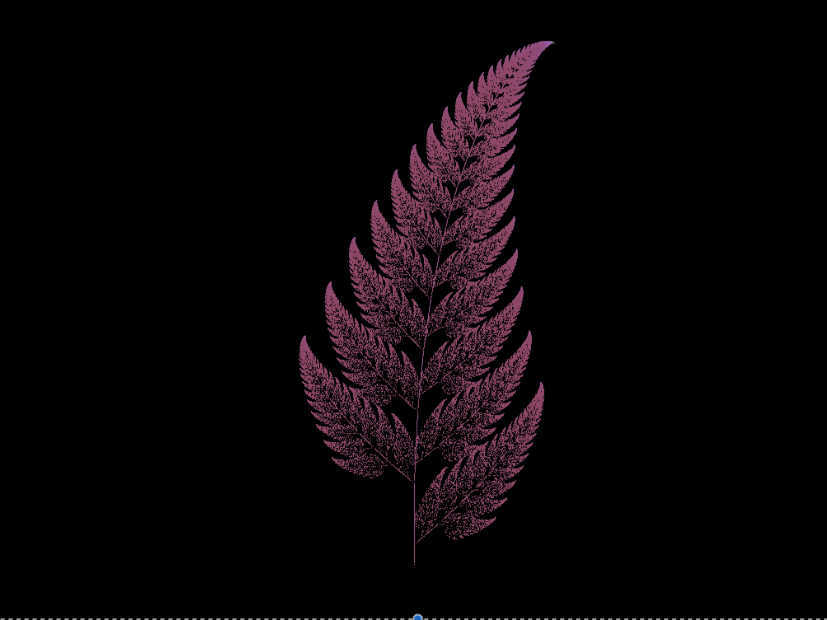
\includegraphics[width=\textwidth]{img/Theory/Fractals/Leaf.png}
                
                \label{fig:gull}
        \end{subfigure}%
        ~ %add desired spacing between images, e. g. ~, \quad, \qquad, \hfill etc.
          %(or a blank line to force the subfigure onto a new line)
        \begin{subfigure}[b]{0.4\textwidth}
                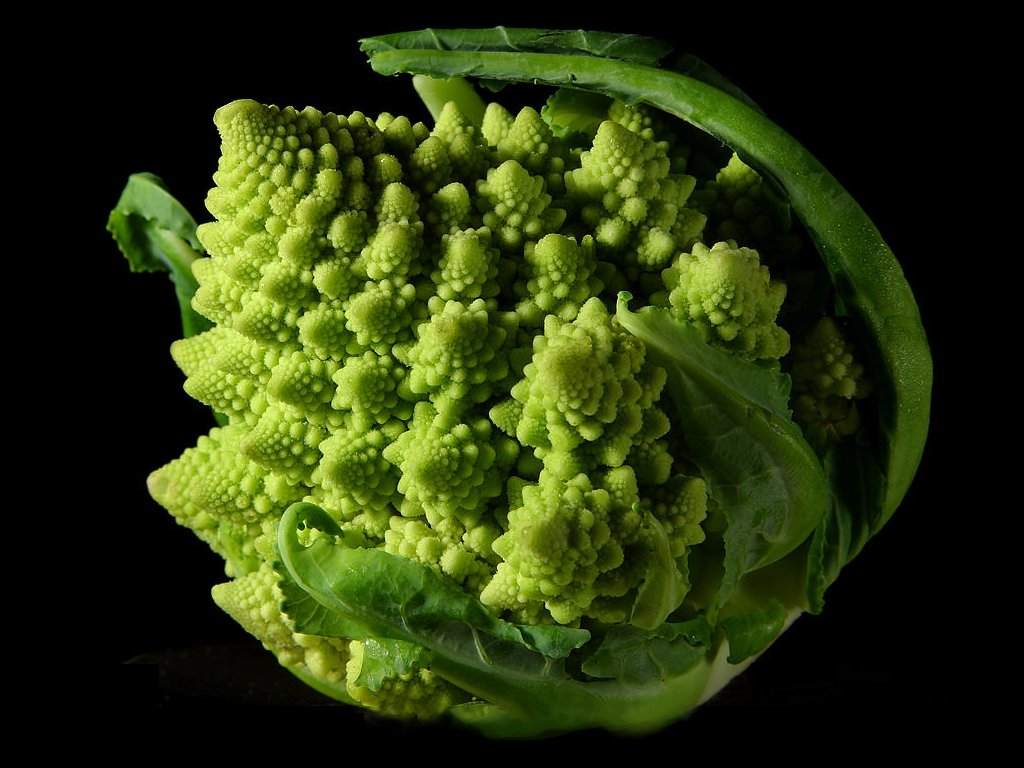
\includegraphics[width=\textwidth]{img/Theory/Fractals/Fractal_Broccoli.jpg}
                
                \label{fig:tiger}
        \end{subfigure}
        \caption{Fractals in Nature}\label{fig:NFractals}
\end{figure}




This idea was applied in maths with the evolution of a new area in this science called fractal mathematics. The objective of this field is to describe this very complex shapes. With really simple rules as repeating a substitution pattern. 

\begin{figure}[htbp]
	\centering
	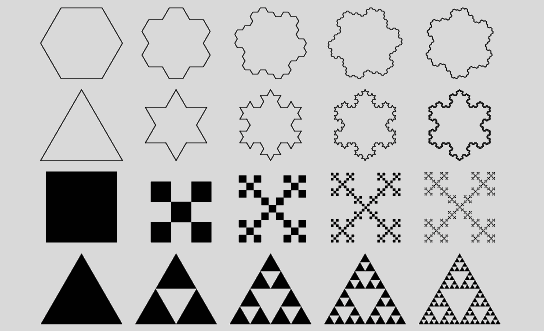
\includegraphics[width=0.9\textwidth]{img/Theory/Fractals/Fractal1_1000.png}
	\caption{Geometric Fractals}
	\label{fig:GFractals}
\end{figure}

In the Figure~\ref{fig:GFractals} there are four examples of Geometric Fractals, with the first five iterations of each one. All of them are built by the substitution of a part of the image by another one. 

The example of the second row is known as the Koch snowflake. In this example, at each iteration, all the line segments are replaced by four segments with 1/3 of the size of the original one with the two in the middle being placed in a angle forming a equilateral triangle with the original line that is removed.

It's clear that the detail that is presented in each iteration increases as the scale changes. To try to mesure this evolution there is the idea of ​​fractal dimension in which the detail in a pattern changes in comparison with the scale in which it is measured (Fractal\_dimension). 

A fractal shape is defined by a recursive algorithm and successive recursions create more detail. There is no theoretic limit to the recursion size and with this a fractal is infinitely detailed. 


% subsubsection fractals (end)



\subsubsection{Cellular Automaton} % (fold)
\label{ssub:cellular_automaton}


It's a model of a system of cells within a grid with a determined shape, each of this cells can be on one of a finite set of states. It evolves during a finite amount of time steps with a set of simple rules according with the state of the neighbouring cells.
The neighbourhood of the cell can be defined in many different ways, the most common is the use of the adjacent cells.

Starting from a line with zeros except the middle cell with one and the following set of rules:

\begin{figure}[htbp]
	\centering
	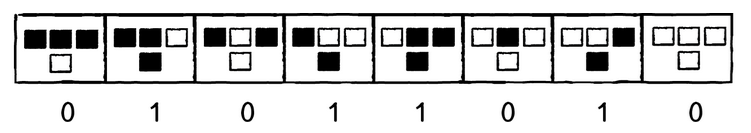
\includegraphics[width=0.85\textwidth]{img/Theory/Cellular_A/Rules.png}
	\caption{Example Production Rules\cite{Shiffman2012}}
	\label{fig:label}
\end{figure}



The Figure~\ref{fig:resultCA} image represents the evolution of one Cellular automaton over time.  In this case, each cell can have one of two states, black or white. Starting from a white line except the middle cell that is black and the presented set of rules.

\begin{figure}[htbp]
    \centering
    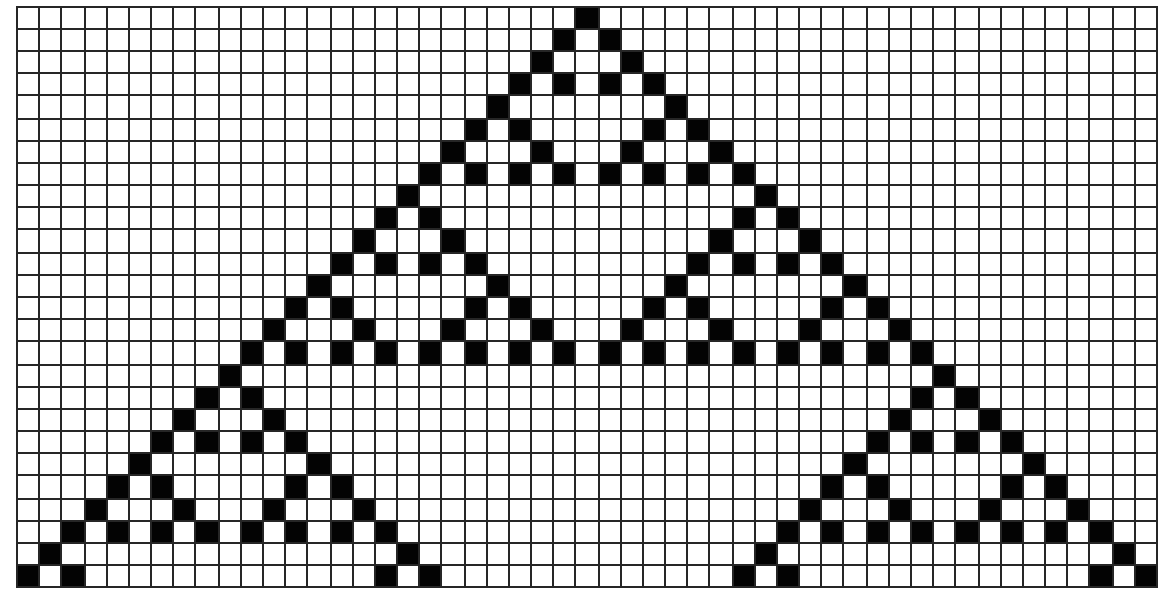
\includegraphics[width=0.85\textwidth]{img/Theory/Cellular_A/Result.png}
    \caption{caption}
    \label{fig:resultCA}
\end{figure}



Each line represents an iteration of the system with the application of the rules. With this set of rules Sierpiński triangle can be reproduced. 



L-Systems
Lindenmayer Systems (L-Systems) are a class of string rewriting mechanisms, originally developed by Lindenmayer as a mathematical theory of plant development.

One Lindenmayer-System, or L-System, is a type of a formal grammar and a string rewriting system that is capable of describe the behaviour of plant cells and model the growth processes of plant development.

It consists of two different parts, one axiom and a set of production rules. The axiom is the starting point of the system, acting as a seed. Then is't applied in this seed the set of production rules, that change the initial string and producing other strings.
This is an iterative process, so after the production of a larger set of strings, the rules can be applied to each one of them wish grows the size of the set even larger.

This L-Systems are used to produce natural growth of vegetation, and the generation of Fractals. 



All the Fractals in the image were generated using L-Systems. 
image from Wolfram MathWorld

In this process, each symbol is associated with a production rule. For instance having $\{a, b\}$ as our alphabet and $\{a=>ab, b=> bab\}$. From a starting axiom \emph{aba}, and the application of the rules we have:\\
\\
\centerline{a b a}
\centerline{ab bab ab}
\centerline{ab bab bab ab bab ab bab}
\centerline{ab bab bab ab bab bab ab bab ab bab bab ab bab ab bab bab ab bab}
\\
\\
This is an example of the evolution of one system. Note that the space between the symbols are just for readability.

% subsubsection cellular_automaton (end)

\subsubsection{Shape Grammars} % (fold)
\label{ssub:shape_grammars}


Shape Grammars can be considered grammars for design. In stead of having symbols or letters as components of the alphabet, they have shapes that can by in 2D or 3D. So the rules are constructed with this shapes, and specify the evolution of the system. With this process, similar to the L-Systems explained before, the shape starts small and simple and can evolve to one big and/or complex shape.

The process is performed in two steps, the recognition of a shape and the replacement according to the rules that are previously defined. 

The following images exemplify one shape grammar, with one rule and the evolution of the application of this rule to the shapes iteratively.



In this image, it's shown that from very simple initial shape, can be generated a complex from with a few iterations.




This is applied to the generation of buildings in the CityEngine system, using 3D blocks.





The figure on the right shows a simple building that I modelled using CityEngine and it's CGA Shape Grammar. But CGA is powerful enough to model much more complex buildings like the one at the bottom.

 













% subsubsection shape_grammars (end)




\subsubsection{Noise} % (fold)
\label{ssub:noise}


"To generate irregular procedural textures, we need an irregular primitive function,
usually called noise." It's a pseudorandom function that gave the goal to break the monotony of a pattern and make it look more random.
Perlin Noise is the most known and used noise function. It was created by Ken Perlin, for the movie Tron 1982 with the aiming to generate natural looking textures.
With this pseudorandom function, it's generated a sequence of values that are interpolated to generate a coherent noise. With the composition of several layers of this noise it's build a texture that look natural and with fractal like structure.




 For instance, the image above shows the result of six noise functions with different frequencies and amplitudes. And the sum of all this functions is the following.

``You may even imagine that it looks a little like a mountain range."

Source: \url{http://freespace.virgin.net/hugo.elias/models/m_perlin.htm}



% subsubsection noise (end)


\subsubsection{Tiling} % (fold)
\label{ssub:tiling}

A common solution to give realism to 3D objects is the application of textures. One problem is that this textures takes a lot of memory. To work around this problem an easy solution is to have a small texture piece, a tile, and repeat throughout the objects. And this is called tiling. Or as defined in Wolfram: ``A plane-filling arrangement of plane figures or its generalisation to higher dimensions.".  This means, the result constructing a plane from a finite set of ``tiles". 
If this technique is use naively commonly results in not very homogeneous textures, it depends much on the set of tiles that are used. If the borders of all the tiles are the same the result is always homogeneous. But if the borders are very different the chances to have a not uniform texture rises. This example from \cite{ProcWorld} shows how a bad structured tiling system produces a not homogeneous texture.  





To make uniform planes, the boundary of each tile must be coherent, i. e., the borders of connecting tiles have to match. Given a single tile, the so-called first corona is the set of all tiles that have a common boundary point with the tile (including the original tile itself). From that, the simple method to create a homogeneous texture is to connect each tile with one that belongs to it's first corona.
The easy, most simple solution is to make sure that all the tiles have the same borders all around. With this property it's guaranteed that any created texture will be homogeneous. But this solution doesn't provide much irregularity and the results present repeating patterns. 


Wang Tiles is a solution named after Mr Hao Wang, that predicted that tiling was not possible. This process allows tiling with an arbitrary number of different vertical and horizontal borders and from that calculate the set of tiles that are needed to create a full texture without inconsistencies. 



As you might have noticed, the inner content of the tiles are not a problem. As we are trying to create the uniform textures by arranging this smaller pieces only the borders matter, so we can create a set of tiles with the same borders and whatever inner content we want. With this technique the result can be much more irregular. 



Corner Tiles \cite{LD06AWTCECC}:
One alternative to Wang tiles with the points to be coloured.
The vanilla wang tiles have problems in the diagonals that are not taken into account. They are the confrontation between four tiles which leads to less homogeneous texture if we the borders don't match. By using the corners, the problem goes to the sides, that despite being larger, are only the confrontation between two tiles and therefore it leads to a more homogeneous texture.

Genetic tile generation:
“The bottom line for me is, Wang tiles are amazing things until you try to use them seriously. They work great for stuff you can synthesise from the ground up. If you are trying to mix samples from real life, get ready for some trouble.”
\url{http://procworld.blogspot.pt/2013/01/tile-genetics.html}


% subsubsection tiling (end)


 \subsubsection{Voxels} % (fold)
 \label{ssub:voxels}
 Voxels

``Voxel is a combination of ``volume" and ``pixel" ". i. e. the equivalent to pixels in 3D. In other words, if a pixel is a tiny square that represents a part of an model in a plane (picture), a voxel is a cube that represents a part of a model in a space.
Because we usually want to model the world, or parts of it, that have three dimensions, it's easier to visualize this models with voxels.

(\dots?)
% subsubsection voxels (end)

% subsection procedural_modelling_techniques (end)


% subsection procedural_generation (end)

%``As ferramentas de CAD existentes estão vocacionadas para uma utilização manual. Infelizmente, a produção manual de grandes quantidades de formas arquitectónicas complexas é muito morosa. A geração procedimental dessas formas é uma das abordagens que permite acelerar substancialmente esse processo. Esta abordagem consiste na construção algorítmica dessas formas, empregando Gramáticas de Formas, L-systems, Autómatos Celulares, etc. Nesta tese pretende a exploração destas técnicas e a sua implementação na ferramenta Rosetta. A avaliação poderá incluir geração de ambientes urbanos, de edifícios e de ornamentação de acordo com um determinado estilo arquitectónico.``

% `` The existing CAD tools are geared for manual use. Unfortunately, the manual production of large amounts of complex architectural forms is very time consuming. Procedural generation of these forms is one of the approaches which considerably speed up this process . This approach is the algorithmic construction of these forms , using grammars forms , L -systems , Automatic Phones, etc. This thesis aims to exploit these techniques and their implementation in Rosetta tool. The assessment may include generation of urban environments , buildings and ornaments according to a certain style arquitectónico.``

%!TEX root = ../report.tex

% 
% Objectives
% 

\section{Objectives (1pg) [NOT DONE]}
\label{sec:objectives}% (fold)

Clearly explain the project objectives.

The objectives of this project is to study the existing approaches to Procedural Generation and to develop a new tool that will be able to generate large amouts of forms efficiently and according to a particular architectural style .



Design and implementation of mechanisms for procedural generation of architectural form , with possible application to the generation of models of urban environments , buildings and ornaments. Implementation of these mechanisms in the Generative Design tool Rosetta.


%``As ferramentas de CAD existentes estão vocacionadas para uma utilização manual. Infelizmente, a produção manual de grandes quantidades de formas arquitectónicas complexas é muito morosa. A geração procedimental dessas formas é uma das abordagens que permite acelerar substancialmente esse processo. Esta abordagem consiste na construção algorítmica dessas formas, empregando Gramáticas de Formas, L-systems, Autómatos Celulares, etc. Nesta tese pretende a exploração destas técnicas e a sua implementação na ferramenta Rosetta. A avaliação poderá incluir geração de ambientes urbanos, de edifícios e de ornamentação de acordo com um determinado estilo arquitectónico.``

% section Objectives (end)
%!TEX root = ../report.tex

% 
% Related work
% 


\section{Related Work (~17pgs)}
\label{sec:related_work}
%%!TEX root = ../../report.tex

\subsection{Template} % (fold)
\label{sub:Template}


% Example citation:
THIS IS A CITATION\cite{Braem2013a}
  
The related work section will highly volatile, and will mostly depend on your kind of thesis. Talk with your supervisor in order to know how to write this part. Don't take the following bullet points as a certain truth.

\begin{itemize}
  \item Most important part of the document. Might be divided in 2/3 subsections.
  \item Might be devised into related work and 
  \item Should cite a wide range of references ~30, search in google, google scholar, mendley, IEEE explorer etc..
  \item Summarized table of solutions.
\end{itemize}

Citations should be mostly :
\begin{itemize}
  \item magazine articles
  \item conferences / workshops
  \item books and technical reports
\end{itemize}
And make sure that your citations follow the following criteria:
\begin{itemize}
  \item Conferences: name and year
  \item workshops: name of the workshop, name of the conference, location and year
  \item Magazines: volume, issue (if possible article pages), publisher.
  \item Books: title, publisher, ISBN, year
\end{itemize}
Websites should be added as footnotes~\footnote{www.google.com}

% Example image:
\begin{figure}[hb!]
  \centering
  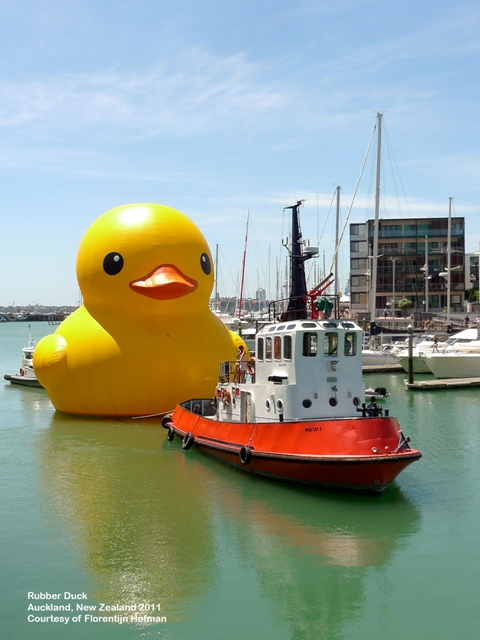
\includegraphics[width=0.95\textwidth]{img/rubberduck.jpg}
  \caption{caption}
  \label{fig:label}
\end{figure}


% subsection Template (end)

%!TEX root = ../../report.tex
\subsection{CityEngine \cite{Parish2001} \cite{Muller2006}}

It's a three-dimensional (3D) modeling software developed by Procedural Inc. (now part of the Esri R&D Center). It's specialized in the generation of 3D urban environments. With the procedural modeling approach, CityEngine enables an efficient creation of detailed and large-scale 3D city models with a lot of control from the user. 

\subsubsection{RoadNetwork} % (fold)
\label{ssub:roadnetwork1}


The first part to procedurally generate a city is to create a road network to become a backbone of the city and provide an overall structure. For that, CityEngine receives as input maps such as land-water boundaries and population
density. From that input a network of highways is created to connect the areas off high density population, and small roads connect to the highways.
This growth process continues until the average area of each lot is the desired one. The system have a default value, bat it can be set by the user to a different one.

To implement this growth process, it's used an L-System, that computes the road network.


\begin{figure}[htbp]
  \centering
  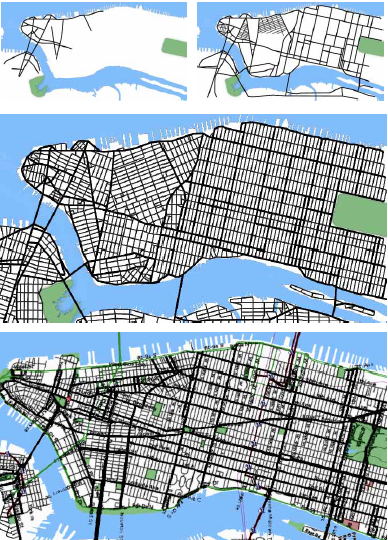
\includegraphics[width=0.5\textwidth]{img/Procedural-Modeling-of-Cities/Capturar.png}
  \caption{Road Map growth}
  \label{fig:city}
\end{figure}

The Figure~\ref{fig:city} shows the evolution of this process in a map of Manhattan. The first two on the top shows the process in different phases during the process, the middle line is the result of the process and the bottom line is the real map of Manhattan for comparison.

% subsubsection roadnetwork (end)Road Network

\subsubsection{Buildings} % (fold)
\label{ssub:buildings1}

To implement the generation of buildings, they created the CGA Shape.

CGA Shape is a Shape Grammar that was introduced by Pascal Muller, Peter Wonka and others, in a paper called ``Procedural Modeling of Buildings''\cite{Parish2001}. It is defined as ``a novel shape grammar for the procedural modelling of CG architecture, produces building shells with high visual quality and geometric detail." To do so, this grammar uses a group of well defined production rules.

This tool allows the user to model buildings with an high control and in different ways. It can be done by text, writing production rules from a shape grammar or with a visual language like Grasshopper 3D, that is nice for simple works but it's impossible to work with a slightly more complex work. 

Mass Modeling
To model a building the first step is to create a mass model of the entire building by assembling basic shapes. With scaling, translation rotation and split applied to basic shapes namely I, L, H, U and T as shown in the Figure~\ref{fig:}.

\begin{figure}[htbp]
  \centering
  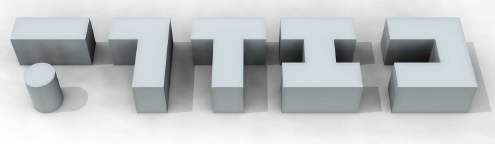
\includegraphics[width=0.95\textwidth]{img/Procedural-Modeling-of-Cities/MassModeling2.png}
  \caption{caption}
  \label{fig:label}
\end{figure}

The next step is to add the roof, from a set of basic roof shapes or general L-Systems.

After that, with the application of the grammar rules in the created mass, it's possible to create complexity to the level that is desired, being able to produce high complex buildings like the one in the following picture.

% subsubsection buildings (end)

\subsubsection{Cities} % (fold)
\label{ssub:Cities1}

The result can be an city like Figure~\ref{fig:bigCity}, with approximately 26000 buildings.

\begin{figure}[htbp]
  \centering
  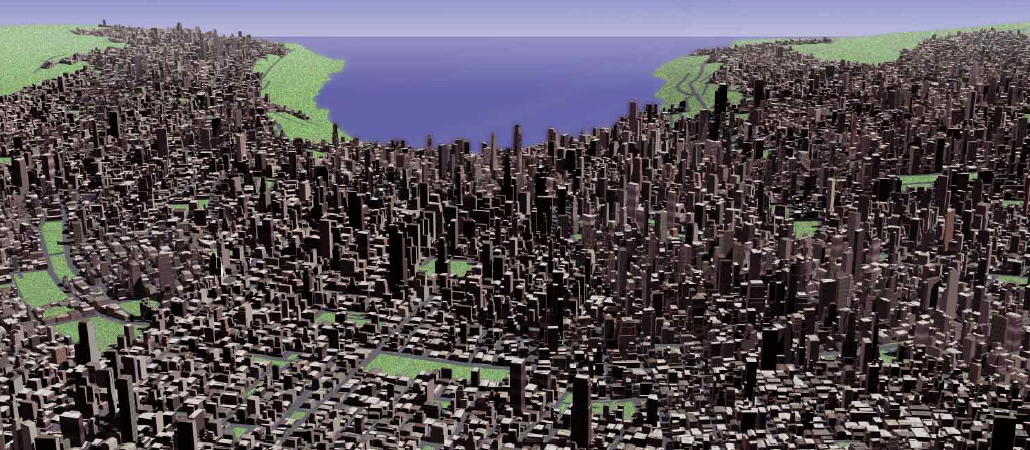
\includegraphics[width=0.95\textwidth]{img/Procedural-Modeling-of-Cities/City.png}
  \caption{City with approximately 26000 buildings.}
  \label{fig:bigCity}
\end{figure}

City Engine results can be imported by Maya, to achieve better results. Like the Figure~\ref{fig:cityMaya}, that represents a ‘virtual’ Manhattan.

\begin{figure}[htbp]
  \centering
  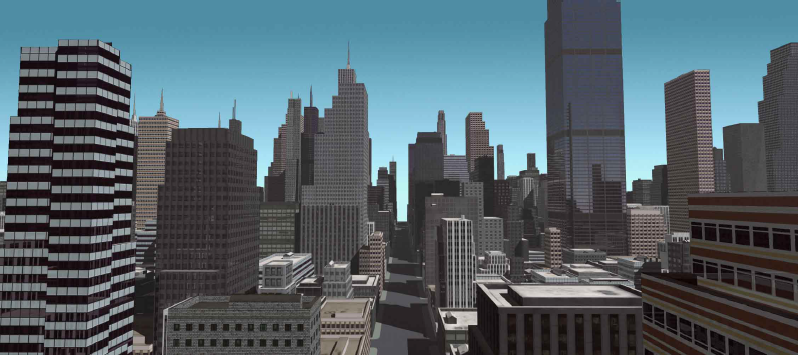
\includegraphics[width=0.95\textwidth]{img/Procedural-Modeling-of-Cities/City_Maya.png}
  \caption{City rendered with Maya.}
  \label{fig:cityMaya}
\end{figure}

% subsubsection subsubsection_name (end)


%!TEX root = ../../report.tex

\subsection{Undiscovered City} % (fold)
\label{sub:undiscovered_city}

In \cite{Greuter2003} Stefan Greuter et al. presented a system that generates in Real-time pseudo infinite virtual cities which can be interactively explored from a first person perspective. In their approach ``all geometrical components of the city are generated as they are encountered by the user." As shown in the Figure~\ref{fig:viewingRange} only the part of city that is inside the viewing range is generate.

\begin{figure}[htbp]
	\centering
	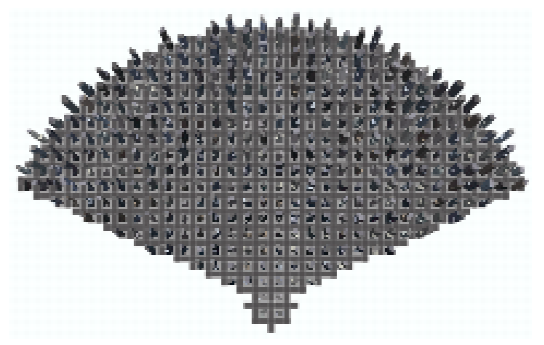
\includegraphics[width=0.85\textwidth]{img/Real-Time-procedural-generation/viewing-range.png}
	\caption{Viewing Range}
	\label{fig:viewingRange}
\end{figure}

\subsubsection{Road Network} % (fold)
\label{ssub:road_network}

The system uses a 2D grid that divide the terrain into square cells. The cells represent proxies for the content that will be procedurally generated. Before the content of each cell is generated, the potential visibility of it is tested, and after that, only the visible cells are filled with content.

After that the roads are created in a uniform grid pattern. This grid does not feel very natural, and in the continuation of the work, this system evolved into a more realistic one with the join of some of the grids to create a less uniform distribution of the buildings.

% subsubsection road_network (end)

\subsubsection{Buildings} % (fold)
\label{ssub:buildings}


To compute the form and appearance of each building, it is used a ``single 32 bit pseudo random number generator seed. The random sequence determines building properties such as width, height and number of floors."
Similar sequences of number result in similar buildings. To avoid that, it is used a a hash function to convert each cell position into a seed.

To generate a building is first is generated a floor plan. To do so, it's randomly selected and merged a set of regular polygons and rectangles, then this is extruded. This is an iterative process, that creates sections from the top to the bottom, by adding more shapes to the the initial shape and extruding as shown in the Figure~\ref{fig:buildings}. Starting from the left, first there is a simple polygon, that is merged with a rectangle and after extrusion, forms the first block that will be the top of the building. After that, another extrusion is made to generate the next block followed by the merge of a rectangle to the floor shape and the generation of a new block and so on.

\begin{figure}[htbp]
	\centering
	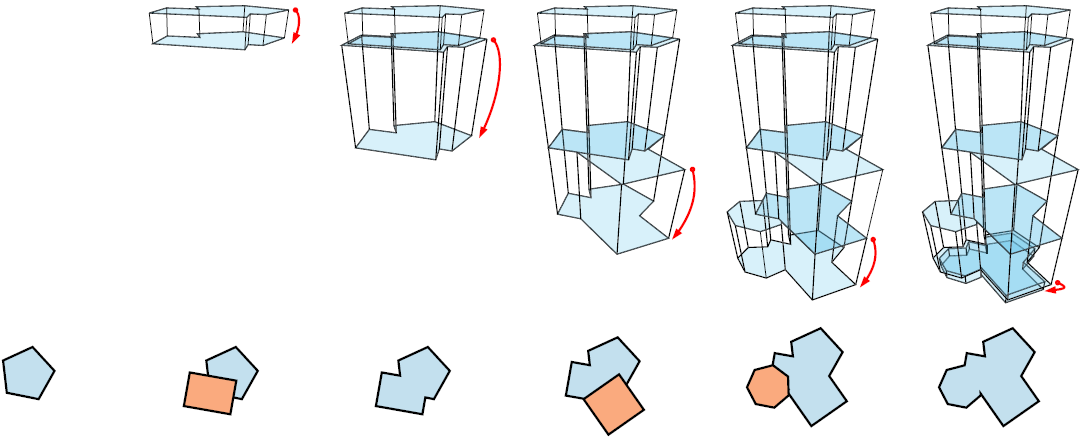
\includegraphics[width=0.85\textwidth]{img/Real-Time-procedural-generation/Building-Generation.png}
	\caption{buildings}
	\label{fig:label}
\end{figure}

With the application of this method very complex architectural forms can be generated, depending only on which forms are selected and the order that is used to merge them.

% subsubsection buildings (end)

% subsection undiscovered_city (end)

%!TEX root = ../../report.tex

\subsection{CityGen } % (fold)
\label{sec:citygen}

CityGen \cite{Kelly2008} it's an interactive system that aims  to ``rapidly create the urban geometry typical of a modern city". The users can interact and control the generation process. The system, like others, is able to generate road networks that act as foundations to the model. It also can generate buildings but can not achieve the complexity and realism of other systems.

\subsubsection{Road Network} % (fold)
\label{ssub:road_network}

CityGen divided this problem in two steps. First the generation of the \emph{Primary Road Network}, and after that, the \emph{Secondary Road Network}. This two steps use different methods to generate the roads.
Undirected planar graphs are used to represent all roads. Two graphs for the Primary roads and one for each zone to store the secondary roads.

\begin{itemize}
	\item[Primary Road Generation] The primary road network uses two graphs, one high level graph that correspond directly to the primary road intersections. It represents the topological structure of the city by it's primary roads, and connections between them. The user is allowed to manipulate this high level graph, to change the high level structure ("topography of the primary road network") of the city .

There is also the low level graph that is generated from the other one, and defines the real path that the roads have in the terrain. It have the same nodes as the first graph and many more, that indicate the points on the terrain which the road passes.

To generate the low level graph it is used ``sampling, plotting and interpolation processes".
\end{itemize}

\begin{figure}[htbp]
	\centering
	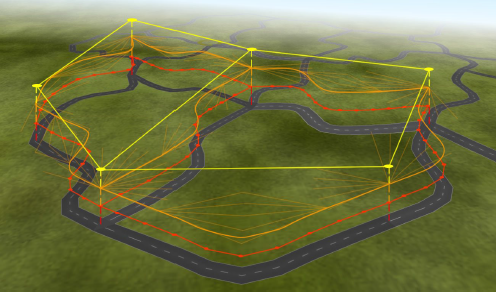
\includegraphics[width=0.85\textwidth]{img/CityGen/RoadGraphs.png}
	\caption{The lighter graph is the High level graph, and the evolution to the darker Low-level graph }
	\label{fig:graphs}
\end{figure}

\begin{itemize}
	\item[Secondary Road Generation] The author defined city cells as districts, that are the areas of terrain that are enclosed by primary roads. The secondary road network is generated inside this cells using a growth based algorithm similar to the L-Systems technique as shown in Figure~\ref{fig:graphs2}.
\end{itemize}


\begin{figure}[htbp]
	\centering
	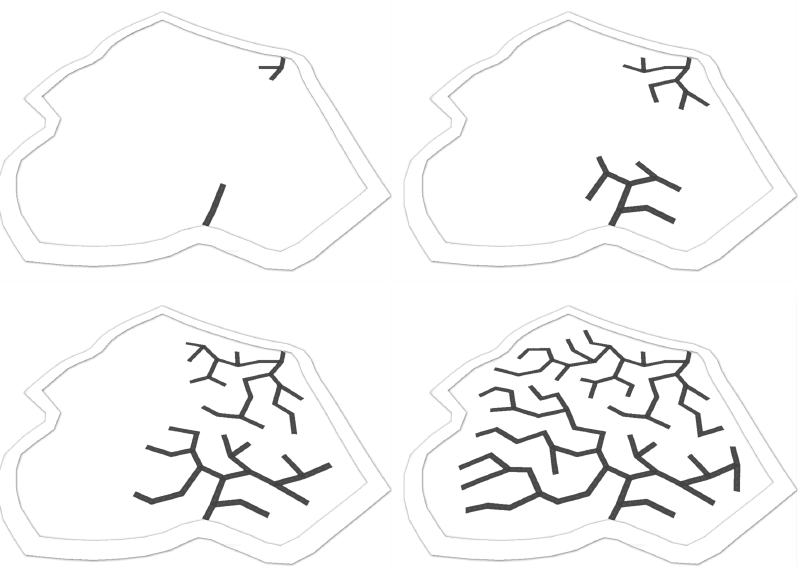
\includegraphics[width=0.85\textwidth]{img/CityGen/SecondaryRoadGrowth.png}
	\caption{}
	\label{fig:graphs2}
\end{figure}

% subsubsection road_network (end)

\subsubsection{Buildings} % (fold)
\label{ssub:buildings}

This system generates buildings also. Each building is created in lots that are identified after the extraction of enclosed regions, called blocks, from the secondary graph. Lots that don't have direct access to the roads are excluded.

Based on the type of block the building footprints are created. After that building geometry is generated by extruding the footprint. The height of each is determined by a height parameter and a noise factor that can be also manipulated. A block is shown in the Figure~\ref{fig:primitiveShapes}, with only primitive shapes.

\begin{figure}[htbp]
	\centering
	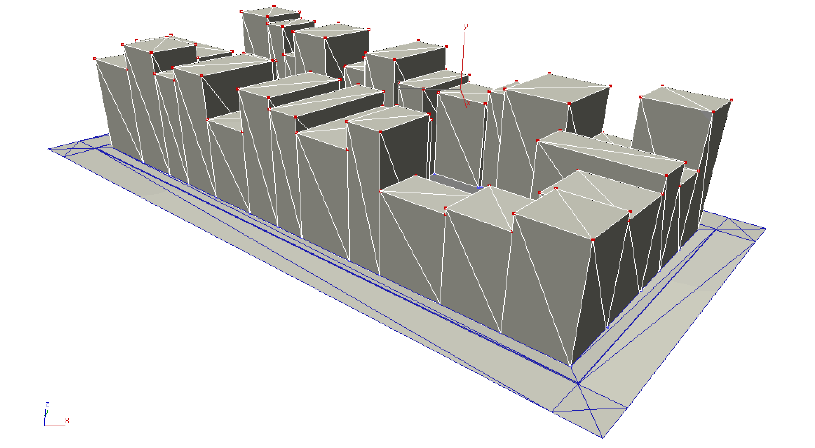
\includegraphics[width=0.85\textwidth]{img/CityGen/BockPrimitiveShapes.png}
	\caption{Primitive Shape Buildings}
	\label{fig:primitiveShapes}
\end{figure}

With this primitive shapes, CityGen uses ``advanced materials with shaders to simulate additional geometry".

% subsubsection buildings (end)

% subsection citygen (end)


%!TEX root = ../../report.tex

\subsection{Inverse Design [NOT DONE]} % (fold)
\label{sub:inverse_design}


In \cite{Vanegas2009} it is presented a different solution from the others already presented.
It's described a framework that enables high level control of the modelling process. It ``provides a mechanism to interactively edit urban models". They apply inverse design to solve the problem of output control. From an existing model, the user can specify high level indicators that describe the desired output and the system change the underlying rules and parameters to get the result as close as possible to the desired.
As the Figure~\ref{fig:loop} shows, the user can change the ``low level" parameters and the ``high level" indicators to control the final output of the system.

\begin{figure}[htbp]
	\centering
	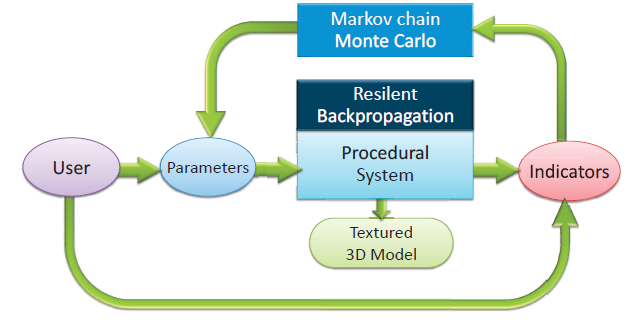
\includegraphics[width=0.95\textwidth]{img/Inverse_Design/TheLoop.PNG}
	\caption{System Pipeline \cite{Vanegas2009}}
	\label{fig:loop}
\end{figure}

This framework uses the indicators as a goal to optimize the parameters. To calculate the values for the parameters they used a version of Monte Carlo Markov Chains (or MCMC) and Resilient Back Propagation.


They implemented a urban procedural engine ``similar to previous city-level procedural modelling work". It was inspired by urban planners, that use the place types concept to represent coherent design patterns of buildings and streets. 


With this approach, the authors claim two main advantages, \emph{Abstraction} and \emph{Interactivity}. They argue that this solution allows urban planners and designers to work at a high level of abstraction, enabling users to manipulate place types, parameters and indicators to create the 3D model they want without wasting time with low level tasks as implementation of low level rules or parameter tuning.
At the same time this approach enables the users to interactively manipulate very complex indicator targets with a ``sophisticated enough" methodology to map target indicators to input low level parameters.


With their teilored version of MCMC and back-propagation they are able to support complex indicators ``enabling control beyond global shape, sush as by high-level semantics and indicators'', and by considering the procedural model as a black box there aren't any limitations to the used grammar.


% \subsubsection{Overview} % (fold)
% \label{ssub:overview}

% A system $P$ produces a geometry $G$ based on \emph{m} input parameter values $\Phi = \{\phi_1,\dots,\phi_m\}$ that is evaluated by an indicator measurement system $I$ which produces a set $\Gamma = \{\gamma_1,\dots,\gama_n\}$ of \emph{n} indicator values.


% % subsubsection overview (end)


% \subsubsection{Inverse Design} % (fold)
% \label{ssub:inverse_design}

% $\Gamma$ - Indicator Values

% $\Phi$ - Input Parameters

% $\Gamma*$ - Target Indicator Values

% $\Phi*$ - Target Parameter Values (specification is optional)


% % subsubsection inverse_design (end)


% \subsubsection{Urban Procedural Model} % (fold)
% \label{ssub:urban_procedural_model}



% subsubsection urban_procedural_model (end)


(\dots)

% subsection inverse_design (end)


%!TEX root = ../../report.tex

\subsection{CityBuilder} % (fold)
\label{sub:citybuilder}


CityBuilder is a system introduced by Watson et. al in \cite{Lechner2003} and \cite{Report2004} ``Procedural City Modeling" and ``Procedural Modeling of Land Use in Cities"}. 
It aims to be self automated to minimize necessary input, only needs the terrain description. Although it allows some other input from the user to give some interaction and control. 
To achieve that, it uses agent based simulation to create a system of agents and behaviours that can model specific entities of a city as developers, planning authorities and road builders. The set of rules for each agent is small to achieve a simple behaviour. With that, they what to make their ``model extendible not only in regard to the types of structures that are produced but also in describing the social and cultural influences prevalent in all cities."

\subsubsection{Road Network} % (fold)
\label{ssub:road_network}
The road network is designed by the agents based on the input terrain description wish will describe the height map and forbidden areas for roads, as water. 
The user can specify that the roads must follow a pre-established gridded pattern, or give the freedom to network to grow more organic. The image presents this two options and a combination of the two with a centre with a gridded pattern ant organic surroundings.


There are two types of road building agents, the extenders and the connectors.

The extenders search the area around exiting developments to look for areas that are not being served by any road to expand the current road network.

The connectors roam trough existing roads and sampling random points in the road network within a given radius. It tries to reach that point trough the road via a BSF. If it cannot reach or the distance needed is over a threshold value, the agent tries to create a road between these two points.


% subsubsection road_network (end)

\subsubsection{Buildings} % (fold)
\label{ssub:buildings}

This system does not develop buildings, but it's developer agents generate parcels and specify the use of the land. They can identify ``at least nine different types of land usages". They perform the role of urban developers that buy land, request planing permission, build and sell. They track the usage of their lands and specify the parameters to the buildings that can be build there.

% subsubsection buildings (end)

\subsubsection{The City} % (fold)
\label{ssub:the_city}

This system develop an evolving conceptual model of one city, that can represent the growth and evolution of a city through the time. 

% subsubsection the_city (end)

% subsection citybuilder (end)


%!TEX root = ../../report.tex

Building Envelopes
\subsection{Building Envelopes [NOT DONE]} % (fold)
\label{sub:building_envelopes}

Sabri Gokmen in \cite{Gokmen2013} presents a way to create envelope systems for buildings. In this case he had a approach that was inspired in Gotheam morphology and leaf venetian patterns.

This article explains form as described by Johann Wolfgang von Goethe in the late eighteenth century. He started by working on annual plants through the work of Linneaus. Goethe considered the external properties of plants to be the result of an internal principle, idea that was influenced by the prior topological work by Linneaus that classified plants according to their physical characteristics.
For Goethe this external properties are not constant and change over time according to environmental conditions.

Forms in architecture are described as a ``topological entity following an overall schema or as a replication of an exiting type that appears fixed (Garcia, 2010)". It says that architects often work with topologies for various buildings and variations are achieved using topological operations. Adding to this is the idea of parametric design to create ``smooth variable systems". This parametric  top-down systems are able to control the overall behaviour of design and have been used to evaluate and adapt performance based approaches in design solutions. ``However this systems are However these systems are ineffective to provide a morphogenetic approach towards design."

Because morphology considers form as the result of a bottom-up process, it is a better method to model growth. Because the form is not defined from start and is the result of the growth process.

Goethe mixed this two ideas namely performance based and morphogenetic approaches. The parametric property is not throughout the system but applied in parts that grow with a morphogenetic approach.

Leaf venetian patterns:
There isn't one certain theory about the guiding principles that support the leaf patterns, there are many theories that try to explain it. One of them is called canalization theory that observes this patterns really as a distribution network, so it depends on the concentration/distributions of auxin producers to efficiently distribute auxin throughout the plant.

Computation of leaf venetian patterns:
The growth algorithm that is presented in this paper is based on the canalization theory. It starts by generating a density map that guides de distribution of auxin sources, that is the second step.
Finally it generates the leaf venetian patterns from the auxin source map.

The generation of the venetian patterns starts by setting root nodes that will be the points from which the patterns will start growing. Then ``at each time step the closest vein node to each auxin source will be defined. Then these nodes will grow towards the average direction influenced by the auxin sources".


% subsection building_envelopes (end)


%!TEX root = ../../report.tex

\subsection{Scene City:} % (fold)
\label{sub:Scene City}

\cite{SceneCity2014}


Scene City is an addon for the 3d application Blender.


“It varies the colors, materials and procedural elements enough to produce a reasonable approximation of a city at a distance, but realism is not a goal, and it does not operate on real data at all.” (http://vterrain.org/Culture/BldCity/Proc/ )

% subsection suicidator_city_generator_ (end)

\subsection{ghostTown:} % (fold)
\label{sub:ghosttown}

http://kilad.net/site/
http://www.kilad.net/GTForum/


It’s a script plugin for 3DS Max from Autodesk.
“Ghost Town is a script that procedurally generates cities and urban environments in only a few clicks, and features a number of options. Such as low or high poly buildings, road layouts, vehicles, trees, facades and an easy to use material and texture system.” (http://cgi.tutsplus.com/tutorials/create-a-detailed-city-with-3d-studio-max-ghost-town--cg-10090)

% subsection ghosttown_ (end)

\subsection{Skyscraper:} % (fold)
\label{sub:skyscraper}

http://www.skyscrapersim.com/index.shtml
Standalone


“Skyscraper aims to be a fully-featured, modular, 3D realtime building simulator, powered by the Scalable Building Simulator (SBS) engine. The main feature SBS provides is a very elaborate and realistic elevator simulator, but also simulates general building features such as walls, floors, stairs, shaftwork and more. Many more things are planned, including gaming support (single and network multiplayer), and a graphical building designer. Skyscraper is written in C++ and uses the OGRE graphics engine, Bullet for collisions and physics, FMOD for sound, the wxWidgets GUI library, and is multiplatform. The current versions aim for a future 2.0 release.” from the official site.

% subsection skyscraper (end)

\subsection{Blended Cities:} % (fold)
\label{sub:blended_cities}

http://jerome.le.chat.free.fr/index.php/en/city-engine/
Addon for Blender

“Blended Cities is an open-source city generator for Blender. it allows to create quickly a large amount of streets and buildings, with various shapes. B.C. fights against squared things : curved streets and odd or cylindric buildings can be created simply, so you can create old towns, not only modern cities.”

% subsection blended_cities_ (end)

%%!TEX root = ../../report.tex

\subsection{Template} % (fold)
\label{sub:Template}


% Example citation:
THIS IS A CITATION\cite{Braem2013a}
  
The related work section will highly volatile, and will mostly depend on your kind of thesis. Talk with your supervisor in order to know how to write this part. Don't take the following bullet points as a certain truth.

\begin{itemize}
  \item Most important part of the document. Might be divided in 2/3 subsections.
  \item Might be devised into related work and 
  \item Should cite a wide range of references ~30, search in google, google scholar, mendley, IEEE explorer etc..
  \item Summarized table of solutions.
\end{itemize}

Citations should be mostly :
\begin{itemize}
  \item magazine articles
  \item conferences / workshops
  \item books and technical reports
\end{itemize}
And make sure that your citations follow the following criteria:
\begin{itemize}
  \item Conferences: name and year
  \item workshops: name of the workshop, name of the conference, location and year
  \item Magazines: volume, issue (if possible article pages), publisher.
  \item Books: title, publisher, ISBN, year
\end{itemize}
Websites should be added as footnotes~\footnote{www.google.com}

% Example image:
\begin{figure}[hb!]
  \centering
  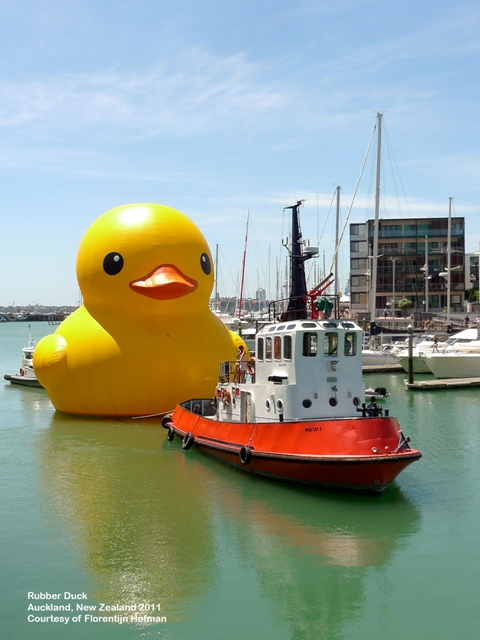
\includegraphics[width=0.95\textwidth]{img/rubberduck.jpg}
  \caption{caption}
  \label{fig:label}
\end{figure}


% subsection Template (end)



%!TEX root = ../report.tex

% 
% Architecture
% 

\section{Architecture}

Lorem ipsum dolor sit amet, consectetur adipisicing elit, sed do eiusmod
tempor incididunt ut labore et dolore magna aliqua. Ut enim ad minim veniam,
quis nostrud exercitation ullamco laboris nisi ut aliquip ex ea commodo
consequat. Duis aute irure dolor in reprehenderit in voluptate velit esse
cillum dolore eu fugiat nulla pariatur. Excepteur sint occaecat cupidatat non
proident, sunt in culpa qui officia deserunt mollit anim id est laborum.
%!TEX root = ../report.tex

% 
% Evaluation
% 

\section{Evaluation (1/2pgs)  [NOT DONE]}
\label{sec:evaluation}

% Explain how you are going to show your results (statistical data, cpu performance etc). Answer the following questions:
% \begin{itemize}
%   \item Why is this solution going to be better than others.
%   \item How am I going to defend that it is better.
% \end{itemize}
To evaluate this work I will be focus on three points, Realism, Scale and Efficiency. 
First for realism, th

Evaluation method taken from \cite{Kelly} to use as an inspiration
\begin{enumerate}
	\item Realism – Does the generated city look like a real city?
	\item Scale – Is the urban landscape at the scale of a city?
	\item Variation – Can the city generation system recreate the variation of road networks and buildings found in real cities or is the output homogeneous?
	\item Input – What is the minimal input data required to generate basic output and what input data is required for the best output?
	\item Efficiency – How long does it take to create the examples shown and on what hardware are they generated? How computational efficient is the algorithm?
	\item Control – Can the user influence city generation and receive immediate feedback on their actions? Is there a tactile intuitive method of control available or is the control restricted? To what degree can the user influence the generation results?
	\item Real-time – Can the generated city be viewed in real-time? Are there any rendering optimisation techniques applied to enable real-time exploration?
\end{enumerate}

%!TEX root = ../report.tex

% 
% Conclusions
% 

\section{Conclusions  [NOT DONE]}
\label{sec:conclusions}

Wrap up what you wrote.
\newpage
%\appendix
%%!TEX root = ../report.tex

\section{Appendix} % (fold)
\label{sec:attachments}

Appendix files and refs will go here.
Such as your thesis work scheduling. 

\subsection{Work Scheduling Example} % (fold)
\label{sub:work_scheduling}
Simple work schedule is presented in Table~\ref{tab:worktable}. You can do something more fancy link a Gantt chart or whatever.
\begin{table}[H]
  \caption{Work Scheduling}
  \label{tab:worktable}
  \begin{center}
    \begin{tabular}{l|cc}
    \hline

    \hline
    \textbf{Month} & \textbf{Work} \\
    \hline
      February & Do Stuff \\
    \hline
      February & Do Stuff \\
    \hline
      March & Do Stuff   \\
    \hline
      April & Do Stuff   \\
    \hline
      May & Do Stuff   \\
    \hline
      May & Do Stuff   \\
    \hline
      June & Do Stuff   \\
    \hline
      July & Do Stuff   \\
    \hline

    \hline
    \end{tabular}
  \end{center}
\end{table}


% 
% Bibliography
% 
\bibliographystyle{plain} 

% replace example.bib with your .bib
\bibliography{example.bib} 

\end{document}